%% Various commands to be used in the main.tex.
\newcommand{\tabreducedunits}{
\begin{table}[h]
\begin{tabular}{|l|c|c|}
\hline Quantity & Symbol & Relation to SI \\
\hline Length & $r^{*}$ & $r \sigma^{-1}$ \\
\hline Mass & $m^{*}$ & $m M^{-1}$ \\
\hline Time & $t^{*}$ & $t \sigma^{-1} \sqrt{\epsilon / M}$ \\
\hline Temperature & $T^{*}$ & $k_{B} T \epsilon^{-1}$ \\
\hline Energy & $E^{*}$ & $E \epsilon^{-1}$ \\
\hline Force & $F^{*}$ & $F \sigma \epsilon^{-1}$ \\
\hline Pressure & $P^{*}$ & $P \sigma^{3} \epsilon^{-1}$ \\
\hline Velocity & $v^{*}$ & $v \sqrt{M / \epsilon}$ \\
\hline Density & $\rho^{*}$ & $M \sigma^{3} V^{-1}$ \\
\hline
\end{tabular}
\caption{\label{tab: reduced units}Reduced units conversion table. Adapted from \cite{gromacs}.}
\end{table}
}

\newcommand{\LJpotential}{
\begin{equation}
    V(r_\mathrm{rel})=4\epsilon\left[\left(\frac{\sigma}{r_\mathrm{rel}}\right)^{12}-\left(\frac{\sigma}{r_\mathrm{rel}}\right)^{6}\right]
    \label{eqn: LJpotential}
\end{equation}
}

\newcommand{\LJforce}{
\begin{equation}
    \mathbf{F}(\mathbf{r}_\mathrm{rel})=-\epsilon\left(\frac{24 \sigma ^6 }{|\mathbf{r}_\mathrm{rel}|^7}-\frac{48 \sigma ^{12}}{|\mathbf{r}_\mathrm{rel}|^{13}}\right)\hat{n}
    \label{eqn: LJforce}
\end{equation}
}

\newcommand{\Verletalgo}{
\begin{equation}
\begin{aligned}
\mathbf{x}(t+\Delta t) &=\mathbf{x}(t)+ \mathbf{v}(t)\Delta t+\frac{{\Delta t}^{2}}{2} \mathbf{F}(\mathbf{x}(t)) \\
\mathbf{v}(t+\Delta t) &=\mathbf{v}(t)+\frac{\Delta t}{2}(\mathbf{F}(\mathbf{x}(t+\Delta t))+\mathbf{F}(\mathbf{x}(t))
\end{aligned}
\label{eqn: Verlet algorithm}
\end{equation}
}

\newcommand{\Verletalgomod}{
\begin{equation}
\begin{aligned}
\mathbf{x}(t+\Delta t) &= \left( \mathbf{x}(t)+ \mathbf{v}(t)\Delta t+\frac{{\Delta t}^{2}}{2} \mathbf{F}(\mathbf{x}(t))\right)\text{mod }{L}  \\
\mathbf{v}(t+\Delta t) &=\mathbf{v}(t)+\frac{\Delta t}{2}(\mathbf{F}(\mathbf{x}(t+\Delta t))+\mathbf{F}(\mathbf{x}(t))
\end{aligned}
\label{eqn: Verlet algorithm modulo}
\end{equation}
}

\newcommand{\figPBC}{
\begin{figure}[h]
\centering
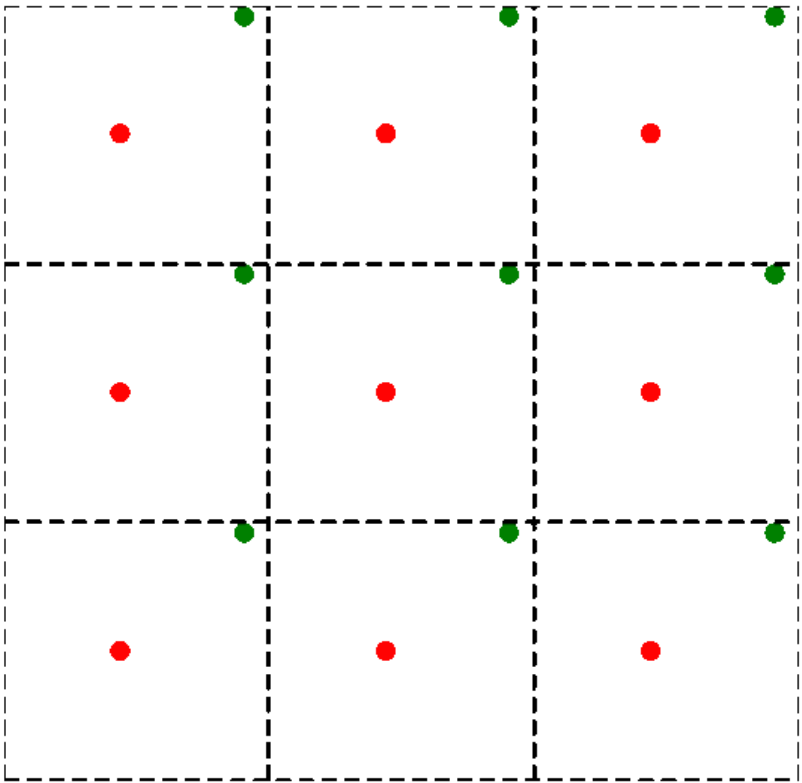
\includegraphics[width=0.55\linewidth]{images/PBC.png}
\caption{Schematic of the simulation domain with two atoms being repeated to infinity in all directions. Adapted from \cite{tudelftnotes}.}
\label{fig: PBC}
\end{figure}
}

\newcommand{\mirrorimage}{
\begin{equation}
    \mathbf{r}_\mathrm{rel}=\left(\left(\mathbf{x}_i-\mathbf{x}_j+L/2\right)\text{mod }L\right)-L/2
    \label{eqn: mirrorimage}
\end{equation}
}

\newcommand{\figmirrorimage}{
\begin{figure}[h]
\centering
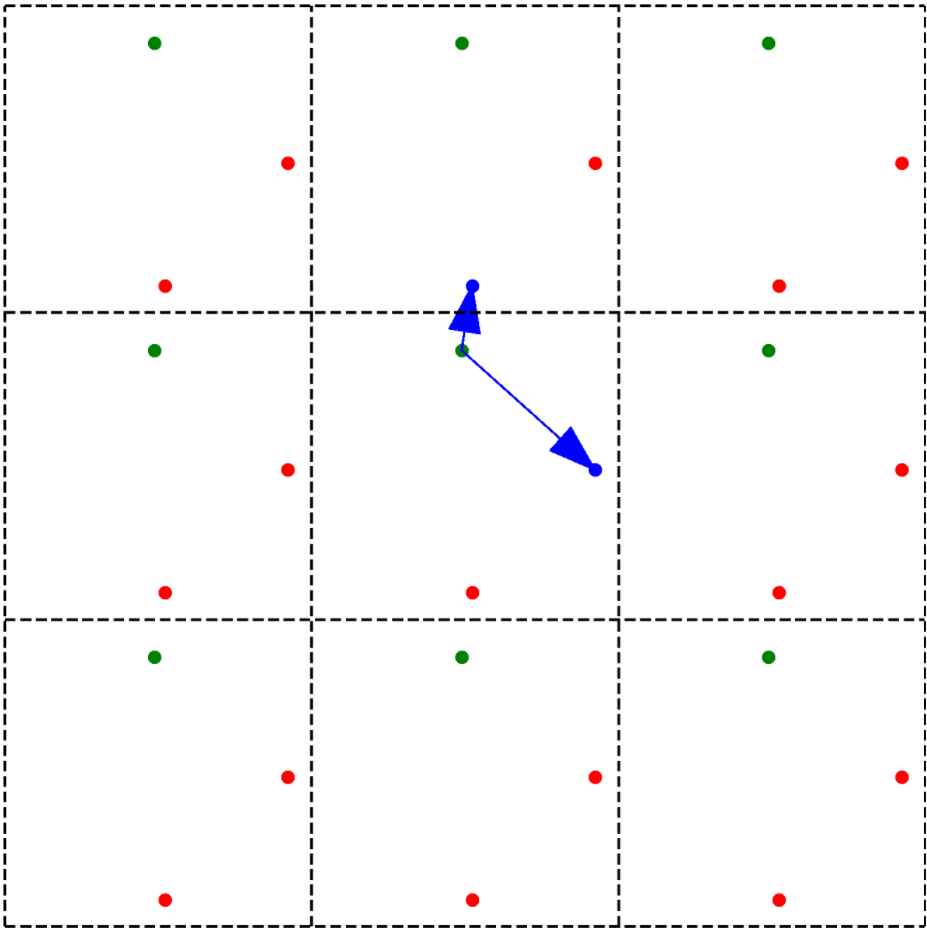
\includegraphics[width=0.55\linewidth]{images/mirrorconvention.png}
\caption{Schematic of the simulation domain with three atoms being repeated to infinity in all directions. The blue arrows denote the interaction pair that corresponds to the closest mirror image. Adapted from \cite{tudelftnotes}.}
\label{fig: mirrorimage}
\end{figure}
}

% UNUSED
\newcommand{\KEtot}{
\begin{equation}
    K_\mathrm{tot} = \sum_{i=1}^{N} \frac{mv_i^2}{2}
    \label{eqn: Total Kinetic Energy}
\end{equation}
}

%UNUSED
\newcommand{\PEtot}{
\begin{equation}
    V_\mathrm{tot} = \frac{1}{2}\sum_{i=1}^{N} V(r_{\mathrm{rel},i})
    \label{eqn: Total Potential Energy}
\end{equation}
}

\newcommand{\PEequalKE}{
\begin{equation}
E_{tot} = V_{tot} + K_{tot}, \quad \frac{dE_{tot}}{dt}=0.
\label{eq:econs}
\end{equation}
}

\newcommand{\pressure}{
\begin{equation}
\frac{\beta P}{\rho}=1-\frac{\beta}{3 N}\left\langle\frac{1}{2} \sum_{i, j} r_{i j} \frac{\partial U}{\partial r_{i j}}\right\rangle
\label{eqn: pressure}
\end{equation}
}

\newcommand{\paircorr}{
\begin{equation}
g(r)=\frac{2 V}{N(N-1)} \frac{\langle n(r)\rangle}{4 \pi r^{2} \Delta r}
\label{eqn: pair correlation function}
\end{equation}
}

\newcommand{\rescaling}{
\begin{equation}
\lambda=\sqrt{\frac{(N-1) 3 k_{B} T_D}{\sum_{i=1}^{N} m v_{i}^{2}}}
\label{eqn: rescaling}
\end{equation}
}




%%%%% REDUCED UNITS %%%%%
\newcommand{\REDUCEDLJpotential}{
\begin{equation}
    V^*(r^*_\mathrm{rel})=4\left[\left(\frac{1}{r^*_\mathrm{rel}}\right)^{12}-\left(\frac{1}{r^*_\mathrm{rel}}\right)^{6}\right]
    \label{eqn: REDUCED LJpotential}
\end{equation}
}

\newcommand{\REDUCEDLJforce}{
\begin{equation}
    \mathbf{F}^*(\mathbf{r}^*_\mathrm{rel})=-\left(\frac{24}{|\mathbf{r}^*_\mathrm{rel}|^7}-\frac{48}{|\mathbf{r}^*_\mathrm{rel}|^{13}}\right)\hat{n}
    \label{eqn: REDUCED LJforce}
\end{equation}
}

\newcommand{\REDUCEDVerletalgomod}{
\begin{equation}
\begin{aligned}
\mathbf{x}^*(t^*+\Delta t^*) &= \left( \mathbf{x}^*(t^*)+ \mathbf{v}^*(t^*)\Delta t^*+\frac{{\Delta t^*}^{2}}{2} \mathbf{F}^*(\mathbf{x}(t^*))\right)\text{mod }{L^*}  \\
\mathbf{v}^*(t^*+\Delta t^*) &=\mathbf{v}^*(t^*)+\frac{\Delta t^*}{2}(\mathbf{F}^*(\mathbf{x}^*(t^*+\Delta t^*))+\mathbf{F}^*(\mathbf{x^*}(t^*))
\end{aligned}
\label{eqn: REDUCED Verlet algorithm modulo}
\end{equation}
}

\newcommand{\REDUCEDPEequalKE}{
\begin{equation}
    E^*_\mathrm{tot}=V^*_\mathrm{tot}+K^*_\mathrm{tot}=\frac{1}{2}\sum_{i=1}^{N} V^*(r^*_{\mathrm{rel},i})+\sum_{i=1}^{N} \frac{{v^*_i}^2}{2}
    \label{eqn: REDUCED Total energy conserved}
\end{equation}
}

\newcommand{\REDUCEDpressure}{
\begin{equation}
\frac{P^*}{\rho^*T^*}=1-\frac{1}{3 N T^*}\left\langle\frac{1}{2} \sum_{i,j} r^*_{i j} \frac{\partial U^*}{\partial r^*_{ij}}\right\rangle
\label{eqn: REDUCED pressure}
\end{equation}
}

\newcommand{\REDUCEDpaircorr}{
\begin{equation}
g^*(r^*_\mathrm{rel})=\frac{2 V^*}{N(N-1)} \frac{\langle n(r^*_\mathrm{rel})\rangle}{4 \pi {r^{*}_\mathrm{rel}}^2 \Delta r^*_\mathrm{rel}}
\label{eqn: REDUCED pair correlation function}
\end{equation}
}

\newcommand{\REDUCEDrescaling}{
\begin{equation}
\lambda^*=\sqrt{\frac{(N-1) 3 T^*_D}{\sum_{i=1}^{N} v{^*_{i}}^{2}}}
\label{eqn: REDUCED rescaling}
\end{equation}
}



\newcommand{\figruntime}{
\begin{figure}[h]
\centering
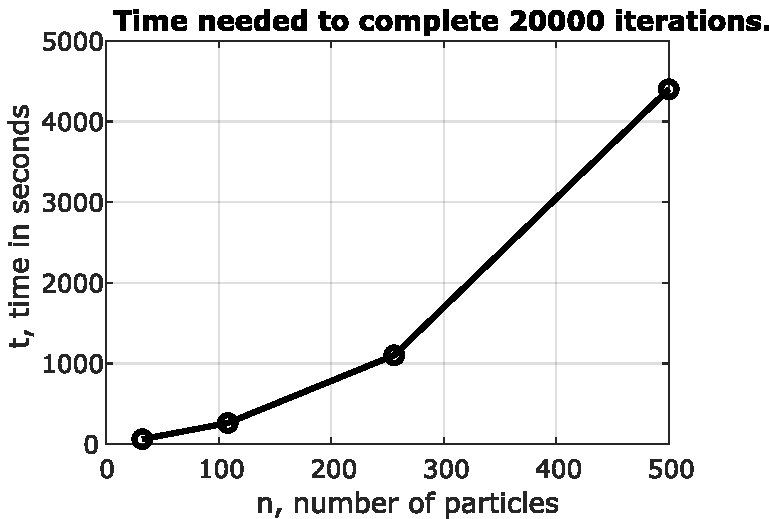
\includegraphics[width=0.75\linewidth]{images/timing.pdf}
\caption{Run-time for simulations for number of particles $n = 32, 108, 256, 500$, each with 20000 iterations. }
\label{fig: runtime}
\end{figure}
}
